\scanpage{12}
\[
\begin{aligned}
v&=\lambda u+\mu&\operatorname{Tr}v&=1\qquad\text{i.e. }\lambda=1\\
v&=u+\mu&\det(\unsure{w|v})&=\underbrace{\det u}+\underbrace{\det\mu.1}_{\mu^2\det1}+\underbrace{\operatorname{Tr}\mu u}_{\mu\underbrace{\operatorname{Tr}u}_{1}}\\
&&&=\alpha+\mu^2+\mu
\end{aligned}
\]

La condition $\underline{\det(v)=\alpha}$ équivaut à

\[
\mu^2+\mu=0\qquad\mu\in\{\underline{0,1}\}\qquad\text{i.e.}\qquad v\in\{u,u'\}
\]

La condition $\det(v)=\alpha'$ équivaut \unsure{à}

\[
\mu^2+\mu+1=0\qquad\text{i.e.}\qquad\mu\in\{\alpha,\alpha'\}
\]

\[
v=u+\alpha,\quad \underbrace{u+\alpha'}_{u'+\alpha}\in S'
\]

\[
\operatorname{Tr}uv=0\qquad\begin{matrix}0&1&\alpha&\alpha'\\&&\alpha^2=\unsure{1|\alpha'}&\end{matrix}
\]

\[
\operatorname{Tr}\underbrace{(u+\alpha)(v+\alpha)}_{uv+\alpha u+\alpha v+\alpha^2}
=\operatorname{Tr}uv+\deleted{\unsure{\alpha}}=\deleted{\unsure{\operatorname{Tr}uv+\alpha}}
\]

\[
\operatorname{Tr}(u+\alpha,v)=\operatorname{Tr}uv+\alpha
\]

\[
\begin{aligned}
&&v&\quad uvu^{-1}\\
\deleted{\operatorname{Tr}v(uvu^{-1})=\operatorname{Tr}((vu)^2u^{-2}}&&v'&\quad u(v)'=u(v')
\end{aligned}
\]

\figure{
\begin{tikzpicture}[scale=.62]\draw[line width=1pt] (0,0)--(1,.03)--(.57,.83)--cycle;\draw (-.07,-.07)--(.62,.78) .. controls (.91,1.02) and (.76,.71) .. (.26,.04)--(1,.03);\draw (.01,.52)--(.62,.78);\end{tikzpicture}}

\diagram{$\begin{array}{c|cccc}\lambda&0&1&\alpha&\alpha'\\\hline \sigma&&&&\end{array}$}

\figure{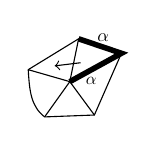
\begin{tikzpicture}[scale=.8]
\coordinate (a) at (0,.72);\coordinate (b) at (.8,1.21);\coordinate (c) at (1.48,.98);\coordinate (d) at (1.05,0);\coordinate (e) at (.26,-.03);\coordinate (o) at (.66,.53);
\draw (a)--(b)--(c)--(d)--(e).. controls (.04,.14) and (.02,.39)..cycle;
\draw (a)--(o)--(b) (o)--(d) (o)--(e);
\draw[line width=2pt] (b)--(c)--(o);
\draw[->] (.83,.83)--(.42,.78);
\node[scale=.65] at (1.19,1.23){$\unsure{\alpha}$};\node[scale=.6] at (1,.54){$\unsure{\alpha}$};
\end{tikzpicture}}

\[
\boxed{\operatorname{Tr}v_0\,u(v_0)=\alpha}\Longrightarrow
\operatorname{Tr}v_{\unsure{i|1|{}}}\,u(v)=\alpha
\quad\text{pour les cinq conjugués de }v
\]

\[
\underset{\operatorname{Tr}(uv)}{\det(u+v)}=
\begin{cases}
\deleted{\unsure{\beta|0}}\alpha&\text{si }\{u,v\}\ \text{\unsure{arête|arêtes}}\\
\alpha'&\text{si }\{u,v\}\ \text{\unsure{coarête|coarêtes|coarêts}}\\
1&\text{si }u=v\\
0&\text{si }u=u'
\end{cases}
\]

\[
\operatorname{Tr}v'\underbrace{u(v')}_{u(v)'}=\alpha
\]

% archive sheet number: 11
